\documentclass[10pt,twocolumn,letterpaper]{article}

\usepackage{cvpr}
\usepackage{times}
\usepackage{epsfig}
\usepackage{graphicx}
\usepackage{amsmath}
\usepackage{amssymb}
\DeclareMathOperator*{\argmax}{argmax}
\usepackage{algorithm}
\usepackage{algpseudocode}
\renewcommand{\algorithmicrequire}{\textbf{Input:}}  % Use Input in the format of Algorithm
\renewcommand{\algorithmicensure}{\textbf{Output:}} % Use Output in the format of Algorithm
\usepackage{color}
\usepackage{graphicx}
\usepackage{subfigure}


% \Cref
\usepackage{hyperref}
\usepackage{cleveref}

\usepackage{tikz}

% Include other packages here, before hyperref.

% If you comment hyperref and then uncomment it, you should delete
% egpaper.aux before re-running latex.  (Or just hit 'q' on the first latex
% run, let it finish, and you should be clear).
% \usepackage[pagebackref=true,breaklinks=true,letterpaper=true,colorlinks,bookmarks=false]{hyperref}

\cvprfinalcopy % *** Uncomment this line for the final submission

\def\cvprPaperID{} % *** Enter the CVPR Paper ID here
\def\httilde{\mbox{\tt\raisebox{-.5ex}{\symbol{126}}}}

% Pages are numbered in submission mode, and unnumbered in camera-ready
\ifcvprfinal\pagestyle{empty}\fi
\begin{document}

%%%%%%%%% TITLE
\title{Integrating Visual and Spatial Information by Graph Convolutional Network \\
for Online Multiple-Object Tracking}

\author{Xiaolong Jiang $^{*}$\\
% Institution1\\
% Institution1 address\\
{\tt Hunan University}
% For a paper whose authors are all at the same institution,
% omit the following lines up until the closing ``}''.
% Additional authors and addresses can be added with ``\and'',
% just like the second author.
% To save space, use either the email address or home page, not both
\and
Peizhao Li \thanks{Equal Contribution}\\
% Institution2\\
% First line of institution2 address\\
{\tt\ Hunan University}
\and
Yanjing Li\\
% Institution2\\
% First line of institution2 address\\
{\tt\ Hunan University}
\and
Xiantong Zhen\\
% Institution2\\
% First line of institution2 address\\
{\tt\ Inception Institute of Artificial Intelligence}
}

\maketitle
\thispagestyle{empty}

%%%%%%%%% ABSTRACT
\begin{abstract}
In this work, we present an end-to-end framework to settle data association in online Multiple-Object Tracking (MOT). Given detection responses, we formulate the frame-by-frame data association as Maximum Weighted Bipartite Matching problem, whose solution is learned using a neural network. The network incorporates an affinity learning module, wherein both appearance and motion cues are investigated to encode object feature representation and compute pairwise affinities. Employing the computed affinities as edge weights, the following matching problem on a bipartite graph is resolved by the optimization module, which leverages a graph neural network to adapt with the varying cardinalities of the association problem and solve the combinatorial hardness with favorable scalability and compatibility. To facilitate effective training of the proposed tracking network, we design a multi-level matrix loss in conjunction with the assembled supervision methodology. Being trained end-to-end, all modules in the tracker can co-adapt and co-operate collaboratively, resulting in improved model adaptiveness and less parameter-tuning efforts. Experiment results on the MOT benchmarks demonstrate the efficacy of the proposed approach.
\end{abstract}

%%%%%%%%% BODY TEXT
\section{Introduction}
Given a video sequence, Multi-Object Tracking (MOT) algorithms generate consistent trajectories by localizing and identifying multiple targets in consecutive frames. Considering its spatial-temporal nature, MOT task is intrinsically complicated for claiming a formidable solution search space. Moreover, the complications of MOT further aggravates with the increasing number of targets, complex object behaviors, and intricate real-life tracking environments.

Aiming at decoupling the combinatorial complications, most trackers solve the object localization and identification separately and lead to two categories of MOT algorithms. On one hand, the Tracking-by-Prediction methods \cite{TbyP1, TbyP2, CyberneticsMine} prioritize object identification by deploying multiple Single Object Trackers (SOTs) on the basis of motion prediction. However, due to the absence of detections, these methods are troubled to adapt to the varying object number because of the object birth \& death (i.e. object entering or leaving the scene). On the other hand, the Tracking-by-Detection methods first localize objects anonymously with detectors, then resolve object identification via data association \cite{OnlineMOTCVPR2014, MulticutTang2017, Cvpr18TwoFoldSiamese}.

In this work, we follow the Tracking-by-Detection strategy. Taking detections as a given, the core of our proposed tracker is its data association module. To achieve online tracking capability, the tracker performs frame-by-frame data associations which can be graphically formulated as Maximum Weighted Bipartite Matching problems. For each pair of consecutive frames, a weighted bipartite graph is constructed involving trajectories in the previous frame and detection responses in the current frame. The matching problem established whereupon is resolved by first generating pairwise affinities as edge weights, then solving the obtained optimization problem to generate the association output.

Accordingly, the data association module starts with generating pairwise affinities. In tracking scenes baffled with target appearance variations and similar distractors, the expressivity and discriminability of the computed affinities is determined by the adopted feature representation method, as well as the distance metric deployed to quantify the affinities. Earlier approaches leverage advanced hand-crafted features \cite{HandAppr1, HandAppr2, HandAppr3} to achieve robust representation. More recently, CNN based deep features are widely exploited \cite{MulticutTang2017, Eccv18BilinaerLSTM, CVPR2017Quadruplet,  PAMI2018DeepApprMOT} instead. Furthermore, a multi-cues strategy has also been practiced to supplement the appearance cue with others \cite{LearnedApprCVPR2010, HandAppr2, TwoStream1}, among which motion is the most vastly adopted \cite{TwoStream2, TwoStream3, TwoStream4, TrackingTheUntrackable, jiang2019model}. On the basis of the encoded feature vectors, hand-engineered distance measures \cite{HandAppr1, BhattacharyyaDist1, BhattacharyyaDist2} are generally utilized to compute the affinity scores. In addition, attempts have also been made to learn metrics that can co-adapt with the feature learning altogether \cite{MWIS2011, TrackingTheUntrackable, Icip2018MOTSiameseLSTM}.

Given the computed affinities, the following optimization problem defined on the weighted bipartite graph is normally configured into a linear assignment formalism and solved with well-designed optimizers or heuristics \cite{BM1WACV2014, BM2ShahCVPR2012}. However, these approaches suffer from tedious designing efforts, prohibitive computation expense, and poor scalability. Particularly, in the presence of frequent object birth \& death, the combinatorial formalism of linear assignment constraints are violated, thus inducing erroneous optimization results which in turn leads to false associations. As a solution, we strive to resolve the optimization problem relying on the function approximation capacity of deep networks in a data-driven way. Nevertheless, this approach is non-trivial to realize. Firstly, although deep neural networks such as CNN and RNN have exceptional feature learning capability, yet their capacities to conduct relational reasoning for data association are limited; Secondly, the varying number of targets give rise to changing dimensionality of the association problem, demanding the otherwise fixed model to be adaptive; Moreover, available data is limited for tracking problem to support the training of heavy models.

Inspired by its graphical formulation of the optimization problem, we observe Graph Neural Network (GNN) \cite{TheGNNModel} is well-suited to solve the problem. By reasoning over non-Euclidean graph data in a message-passing way, the proposed GNN optimization module is endowed with improved relational reasoning capacity and can cope with the varying cardinality problem via the deployments of localized operations. Furthermore, the module is light-weight and converges well. By integrating the aforementioned affinity learning module end-to-end, all parameters in the data association pipeline can co-adapt and co-operate compactly, results in better model adaptiveness, scalability, and efficiency with acceptable model complexity. For the purpose to better optimize the complicated network with diverse modules, we design the multi-level matrix loss which is assembled to enhance the training performance. The main contributions of this work include:
\begin{itemize}
\item We propose an end-to-end framework incorporating affinity learning and optimization modules to solve the data association problem in online multiple-object tracking.
\item We design the optimization module with Graph Neural Network (GNN), which learns to solve the constructed maximum weighted bipartite matching problem in a data-driven way, avoiding excessive algorithm design and parameter tuning efforts.
\item We employ assembled supervision in conjunction with the proposed multi-level matrix loss to ensure the training performance of the end-to-end network composing diverse modules.
\item We demonstrate experimentally that the GNN optimization module improves data association performance, and overall our method yields competitive results with other state-of-the-art trackers on the MOT benchmark.
\end{itemize}

\begin{figure*}[ht]
\centering
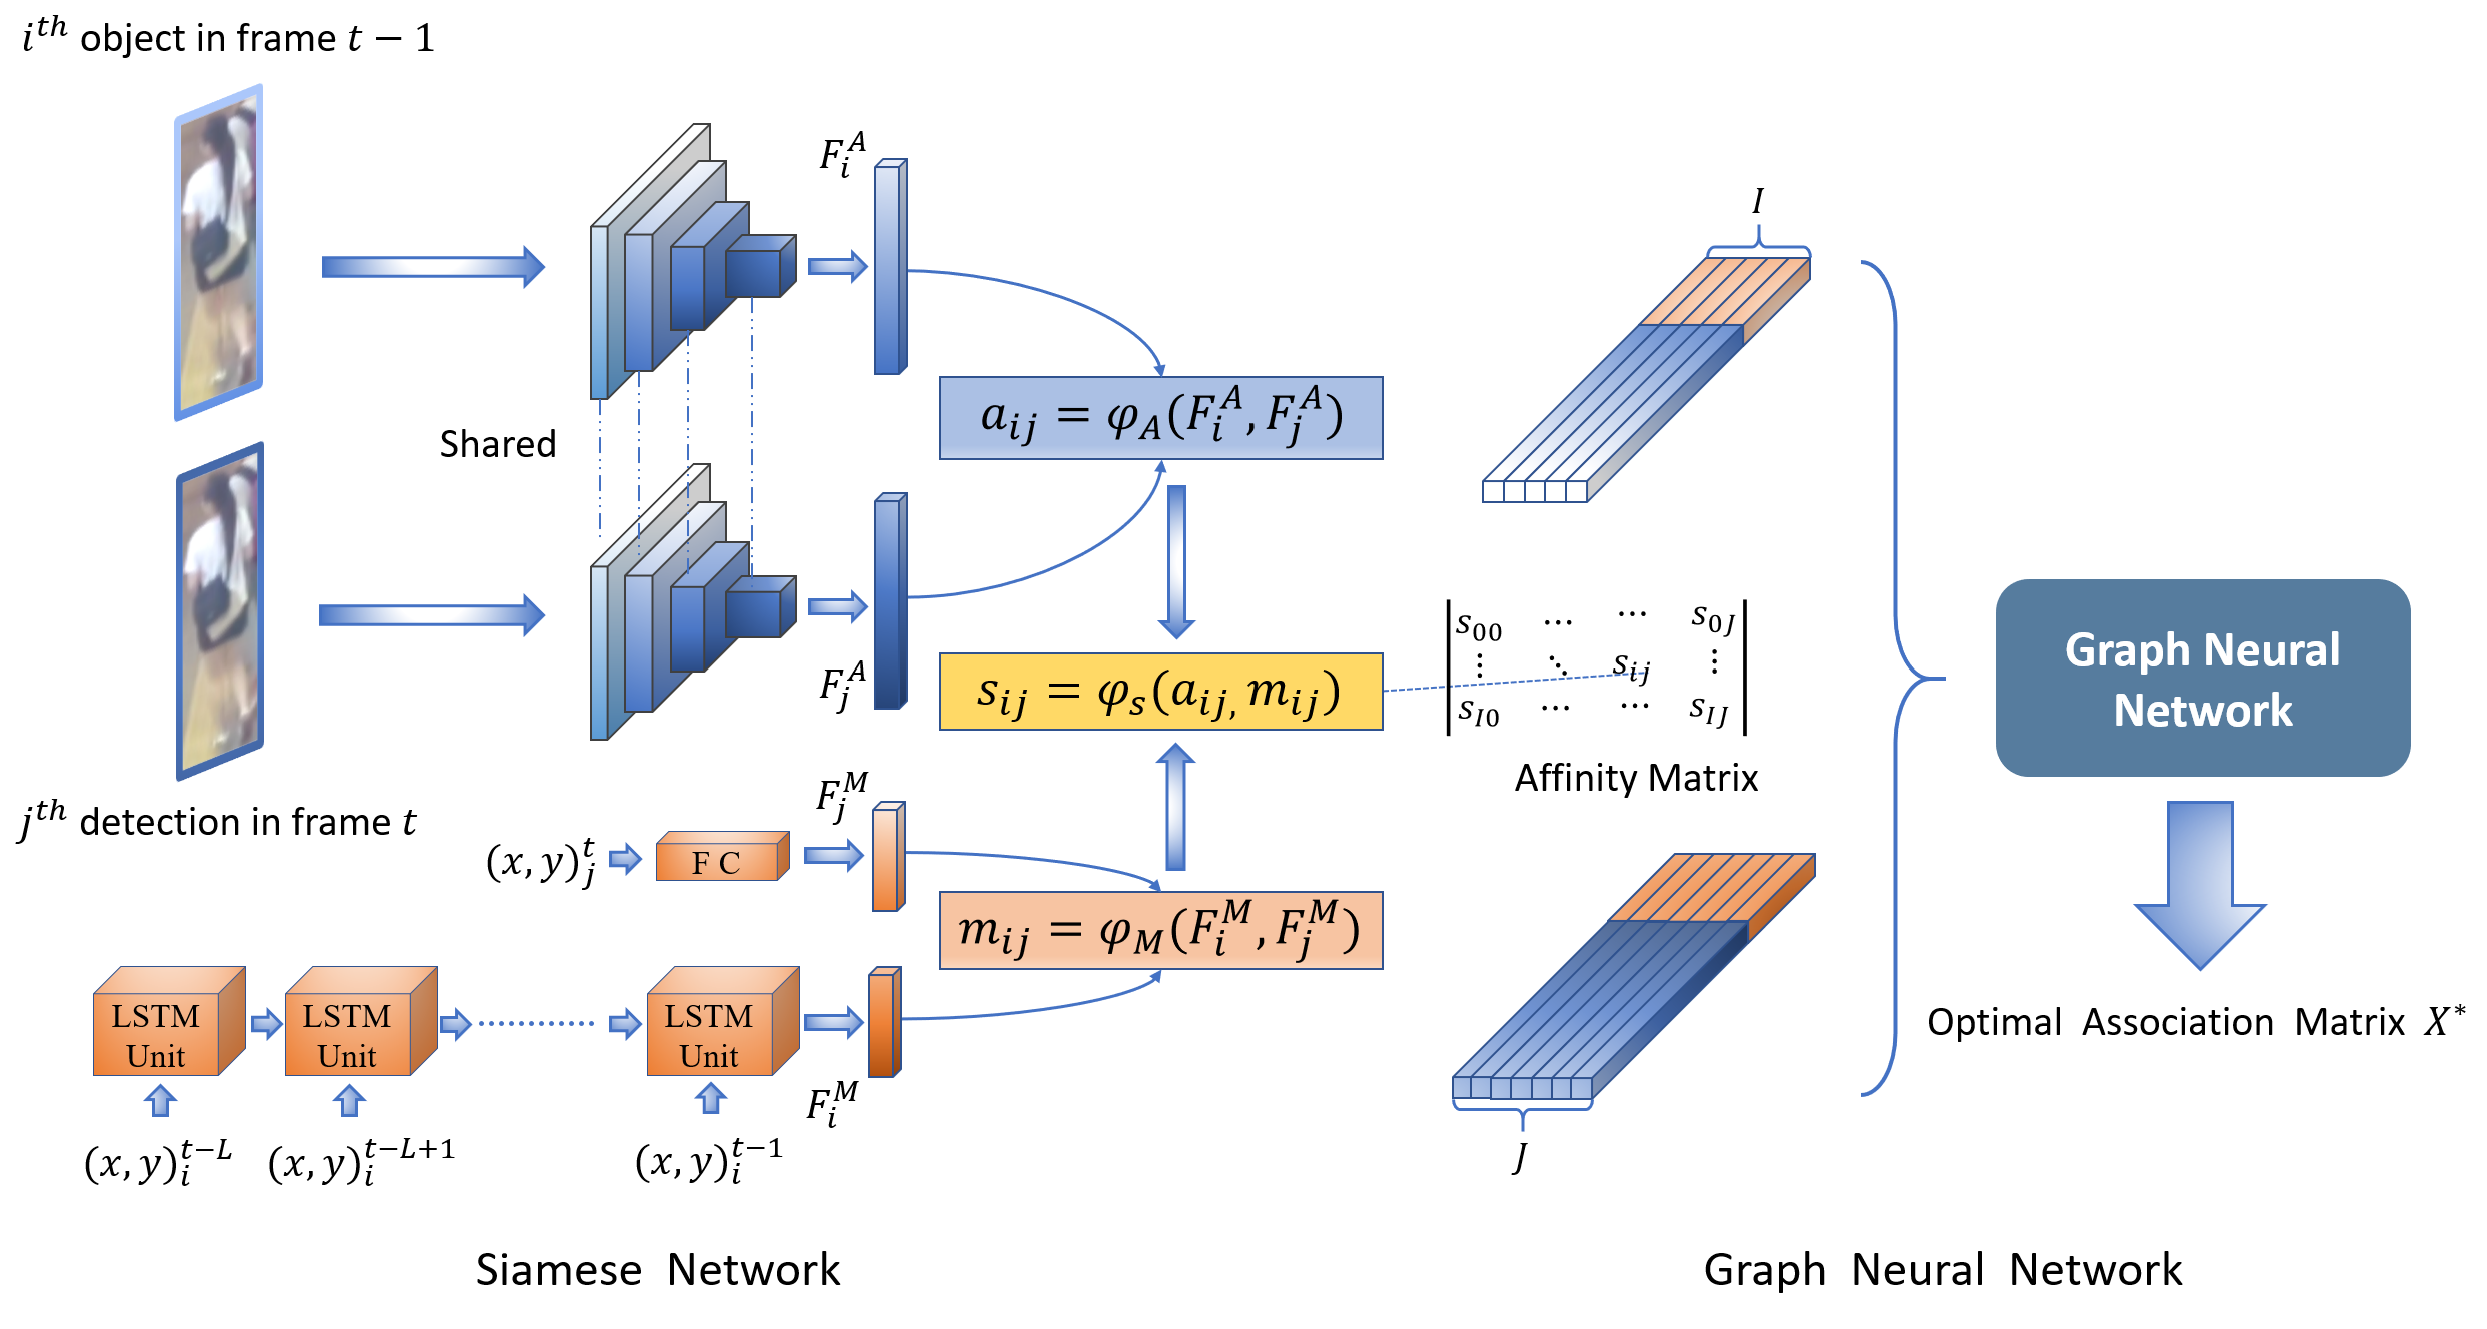
\includegraphics[scale=0.35]{fig/pipeline.pdf}
\caption{Pipeline of our MOT model.
	Inputs are the frame $t-1$, the frame $t$, the object set $\mathcal{O}_{t-1}$ from frame $t-1$ and the detection set $\mathcal{D}_t$ at frame $t$.
	Outputs are tracking results.
	For example, there are four object frame frame $t-1$ and three detections from frame $t$, 
	and their features are extracted and sent into the graph networks.
	Afterwards, data association and missing detections handling are performed.}
\label{fig:pipeline}
\end{figure*}
%-------------------------------------------------------------------------
\section{Related Work}
\textbf{Affinity Computation in Data Association.} Data association is the process of dividing a set of instances into different groups, such that to maximize the global cross-group similarities while maintaining one-to-one association constraint. This fundamental technique exists in various domains that involve correspondence matching \cite{PhdThesisDA}, such as person re-identification \cite{Cvpr2018MTMC, ReIdSurvey, ReIDDA1}, keypoint matching \cite{DLGraphMatching}, 3D reconstruction \cite{PAMI3DReconShah}, action recognition \cite{DA4ActionRecog}, and T-by-D based MOT \cite{LearningByTracking}.

Affinity computation lays the foundation for data association. It provides the similarity measures upon which the maximization is established. In the context of multi-object tracking, pairwise or tracklets-based appearance affinity scores are computed by first extracting reliable feature representations with hand-crafted features \cite{HandAppr1, HandAppr2, HandAppr3, ColorApprCVPR2015, TextureAppr, BrightnessAppr, ICCV2015LocalFlow}, learnable features \cite{ApprAdaBoost, ApprMotionMIL, EnsembleTracking, LearnedApprCVPR2010, LearnedApprECCV2012, LearningToAssociate}, or deep features \cite{PAMI2018DeepApprMOT, DCNNApprFeatureNIPS2013, DeepTrackTIP2016DeepApprFeature}. For the purpose to supplement the appearance cues under severe variations, attempts have been made to jointly investigate multiple cues \cite{LearnedApprCVPR2010, HandAppr2, TwoStream1}. Amongst, motion information is the most widely applied \cite{ApprMotionMIL, DA1, TwoStream2, TwoStream3, TwoStream4, TrackingTheUntrackable}. The similarity between paired feature vectors is quantified by a distance metric such as Euclidean, Mahbolinios or Bhattacharyya distance \cite{HandMadeDistanceMetric1, MilanEnergy, OnlineMOTCVPR2014, HandAppr1, BhattacharyyaDist1, BhattacharyyaDist2}. Moreover, metric learning has also been deployed in \cite{MWIS2011, TrackingTheUntrackable, Icip2018MOTSiameseLSTM} to learn adaptive metric from data. Noteworthily, end-to-end affinity computation has been proposed with deep Siamese architecture \cite{SiameseLeCun, LearningByTracking, TripletLossTrackingEccv18, Cvpr18TwoFoldSiamese, Cvpr2018RASnet, Cvpr2018MTMC, Icip2018MOTSiameseLSTM}.

\textbf{Optimization in Data Association.} Data association can be interpreted as the Set Partition Problem (SPP)\cite{SPP}. In multi-object tracking, this SPP formalism is specialized into the Multi-Dimensional Assignment (MDA) problem, which describes the optimization procedure defined on a k-partite graph to partition object observations into trajectories cross $k$ frames. Offline methods indicate $k>=3$ such that the data association is executed in a batch mode. Such a global association strategy is robust and accurate, yet inevitably introduce NP-hardness and forfeit the real-time tracking capability. Tracklet-based \cite{TrackletsBasedECCV2008, SOTMOT, ECCV18YangMHDualAttention, SOTMOT2} and detection-based \cite{MilanEnergy, NevatiaCVPR2008} methods have been practiced to realize offline multi-object tracking. Differently, online multi-object trackers \cite{BM1WACV2014, BM2ShahCVPR2012, OnlineMOTCVPR2014} perform frame-by-frame associations with real-time tracking capability recovered. Online methods are usually graphically formulated as the Maximum Weighted Bipartite Matching \cite{DLGraphMatching} problem and solved with the Hungarian algorithm \cite{Hungarian}. A variety of other graphical formalisms have also been devised to settle the data association, including Network Flow \cite{ShahNF,PAMI16NF,NF2CVPR2011, DeepNF}, Minimum Cost Multi-cut \cite{Multicut2015CVPR, MulticutECCV2016, MulticutTang2017}, Maximum-weight Multi-Clique \cite{ShahGMMCP2015CVPR}, etc. On the basis of these optimization formulations, attempts have been made to solve the problem in a data-driven manner \cite{DeepNF, DLGraphMatching}. Particularly, in \cite{DeepTracking, ondruska2}, Ondruska et al. initially propose to deploy recurrent neural networks (RNNs) in solving MOT on a primitive level without formal data associations. Following this line of research, in \cite{Milan2017AAAI} Milan et al. established the first end-to-end online multi-object tracking method with explicit data association realized using RNNs.

\textbf{Graph Neural Network}. Common neural networks models are designed to work with Euclidean data as inputs. Graph neural networks, as neural network models operating on non-Euclidean graph data, refers to a structured architecture to conduct graph-to-graph relational reasoning computations \cite{GNNSurvey, DeepMindGNN}. In general, GNN manages to learn complicated semantic information by building them from the lower level in a hierarchical way \cite{DLGoodFellow}. In actualization, this GNN hierarchy is established by aggregating local information from edges to nodes, then to the global level in a message passing manner \cite{MessagePassing}. Over its development in the past decade \cite{GNNOrigin1,GNNOrigin2,GNNorigin3}, GNN models have found far-reaching applications across domains including supervised \cite{GNNSupervised}, semi-supervised \cite{Kipf2017ICLR}, few-shot \cite{GNNFewShot}, and reinforcement learning \cite{GNNReiforcement}, resulted in fruitful well-established networks such as graph convolutional networks \cite{Kipf2017ICLR, MPNN, GAT}, graph-based generative models \cite{MoIGAN, GRNN}, graph-based adversarial learning \cite{GraphSGAN, PeerNets}, etc. Closely related to the proposed work, a few attempts have been taken to settle the Quadratic Assignment Programming (QAP) problem with GNN. In \cite{GNNQAP1}, the general GNN architecture proposed in \cite{GNNorigin3} is adopted to solve the QAP in the context of graph matching. In \cite{GNNCO}, a unique combination of reinforcement learning and graph embedding is realized to resolve the NP-hard combinatorial optimization.

\section{Graph Networks}
The following notions are defined at frame $t$.

\textbf{Trajectory}. A trace formulated by bounding boxes from all the frames between frame 1 and frame $t-1$.

\textbf{Object}. The last bounding box on one trajectory. 
Objects before frame $t$ comprise the object set for frame $t-1$, which is denoted by $\mathcal{O}_{t-1}$.
If the object occurred in frame $t-1$, it is a normal object.
Otherwise, it is a missing object.

\textbf{Detection}. A bounding box in current frame $t$. 
The detection set is denoted by $\mathcal{D}_t$. 

\subsection{Pipeline}
The pipeline is demonstrated in \Cref{fig:pipeline}. 
As shown in \Cref{fig:pipeline}, there are four procedures: feature extraction, graph networks, data association and missing detections handling. 

\textbf{Feature Extraction}.
First, we extract the appearance feataures and the motion features from both objects and detections. 
To be specific, the appearance feature is extracted from a convolutional neural network (CNN).
We generate more discriminative fusion features using visual and spatial relationship among multiple samples.

\textbf{Graph-based Fusion Feature Network}.
Afterwards, graph networks infer the similarity between each object and each detection. 
Each node is associated with the fusion feature of the object/detection,
and each edge that connects the object and the detection is associated with their similarity score.

\textbf{Object Association}.
This procedure outputs the association between the objects and the detections.
The Hungarian algorithm~\cite{kuhn1955hungarian} is used to find the optimal assignments.
Note that we abandon those associations where the object is spatially very far from the detection.

\textbf{Online MOT}.
After the data association procedure, there are still some missing detections.
For those objects that have been missed in the current frame, the single object tracking (SOT) strategy is used to track those missing objects in the current frame,
and associate them with the recovered bounding boxes by SOT with high confidence score.
For those detections that have been missed for a while, we use a detection recovery strategy, which applies a linear motion model to recover those missing detections.

We denote the $i$-th object in $\mathcal{O}_{t-1}$ as $o_i$, 
and the $j$-th detection in $\mathcal{D}_t$ as $d_j$, 
where $a_{i,j}=1$ describes the situation that the detection $d_j$ is associated with the object $o_i$,
and $a_{i,j}=0$ describes the opposite situation.
The assignment set is denoted by $\mathcal{A}_t=\{ a_{i,j} \} ^ {|\mathcal{O}_{t-1}| \times |\mathcal{D}_t| }$, where $| \mathcal{O}_{t-1} |$ and $|\mathcal{D}_t|$ are the numbers of objects and detections, respectively.

The the optimal assignment set can be formulated by 
\begin{equation}
\hat{ \mathcal{A} }_t = 
{\rm argmin}_{\mathcal{A}_t}
\sum_{i=1}^{|\mathcal{O}_{t-1}|}
\sum_{j=1}^{|\mathcal{D}_t|}
a_{a,j}
\mathcal{F} (o_i, d_j),
\end{equation}
\begin{equation} \label{equ:association_constraint}
\mathrm{s.t.}
\sum_{i=1}^{|\mathcal{O}_{t-1}|}
a_{i,j} \leq 1
\ \mathrm{and} \ 
\sum_{j=1}^{\mathcal{D}_t}
a_{i,j} \leq 1,
\end{equation}
where $\mathcal{F}(o_i,d_j)$ denotes the cost between the object $o_i$ and the detection $d_j$.
\Cref{equ:association_constraint} describe that one object can be associated with at most one detection, 
and one detection can be associated with at most one object.
Following the constraints, it is allowed that $\sum_{i=1}^{|\mathcal{O}_{t-1}|} a_{i,j} = 0$ and $ \sum_{j=1}^{|\mathcal{D}_t|} a_{a,j} = 0 $,
which means that detections are associated with no objects,
and objects are missing at current frame.



\subsection{Graph-based fusion feature network}
% GULF, C
Aforementioned, it is insufficient to distinguish different objects by using visual features alone. 
To alleviate this problem, we construct a graph to explore both visual and spatial relationship among multiple samples to generate more discriminative fusion features.

Given a training set $\mathbb{S}$ and a testing set $\mathbb{T}$, we construct a graph $G=(V,E)$, where $V(|V|=N)$ and $E$ are sets of nodes and edges, respectively. 
Each node $v_i$ represents a object image in a training or testing set, and is equipped with a fusion feature vector $f(v_i)$, which is equal to $x_i$ from the path-based feature network initially.
Each edge $e_{ij}$ represents a connection between $v_i$ and $v_j$, and the corresponding weight value $a_{aj}$ indicates the connection strength between them.
Here, we define two kinds of edges: the spatial edge to measure the spatial adjacency between two nodes, and the visual edge to measure the visual similarity between them.
The details are as follows:

Given two nodes $v_i$ and $v_j$, there is a spatial edge $e_{ij}$ between them only if this two nodes are under the same video frame $C_k$. We calculate the weight value $a_{ij}$ as follows:
\begin{equation} \label{equ:weight_value}
a_{ij}=\left\{ \begin{aligned}
& e^{-\alpha*|Dis(v_i, v_j)|}, & v_i \in C_k, v_j \in C_k, \\
& 0, & otherwise, \\
\end{aligned} \right.
\end{equation}
where $\alpha$ is a scale parameter, and $Dis(v_i, v_j)$ measures the spatial distance between $v_i$ and $v_j$.
Here, we adopt the Manhattan distance to calculate the spatial distance $Dis(v_i, v_j)$, which is equal to the average distance between upper left point and lower right point in the format of bounding boxes.
Given a video frame, its bounding boxes is provided in the dataset.
The spatial edge indicates the closeness between two nodes in a frame. 
Concretely, a spatial edge with a large $a_{ij}$ indicates a small distance between $v_i$ and $v_j$, which offer useful spatial relationship information to generate fusion features. 
On the contrary, spatial edge with a small $a_{ij}$ represents a large distance and a weakly spatial correlation between them.
In such case, the introduction of a spatial edge may introduce noises.
There, we set a threshold $\tau_1$, and remove all the spatial edges whose weight values are less than $\tau_1$.

When two nodes $v_i$ and $v_j$ are under two different video frames, the visual edge is employed to measure the visual similarity between them.
Here, the cosine distance is adopted to calculate the weight value $a_{ij}$ as follows:
\begin{equation}
a_{ij}=\left\{ \begin{aligned}
& \frac{v_i \cdot v_j}{||v_i ||_2 ||v_j||_2}, & v_i \in C_{k_1}, v_j \in C_{k_2}, \\
& 0, & otherwise, \\
\end{aligned} \right.
\label{equa:weight_value}
\end{equation}
A visual edge with a large $a_{ij}$ represents a high visual similarity between $v_i$ and $v_j$, which indicates a high probability to connect the same identity by the edge.
On the contrary, a visual edge with a small $a_{ij}$ indicates visual dissimilarity, and is usually invaluable to distanguish different objects.
Therefore, we set a threshold $\tau_2$, and remove all the visual edges whose values are less than $\tau_2$. 

After building the graph, we introduce an adjacency matrix $\boldsymbol{A}$ of graph and its degree matrix $\boldsymbol{D}$, where $D_{ij}=\sum_j A_{ij}$.
GCN can capture information onlyl about immediate neighbors with one layer convolution.
Here, the immediate neighbors refer to those visually similar or spatially close nodes. 
A GCN algorithm operates directly on the graph and induces embedding vector of nodes based on properties of their neighborhoods, which is expressed as:
\begin{equation}
\boldsymbol{F}^{(1)} = \rho(\tilde{\boldsymbol{A}}\boldsymbol{FW}),
\end{equation}
where $\boldsymbol{F}$, $\boldsymbol{F}^(1)$ are initial and updated fusion features, respectively,
and $\boldsymbol{W}$ is a weight matrix.
$\rho$ is an activation function, which is $ReLU$ in our experiments.
Actually, $\tilde{\boldsymbol{A}}\boldsymbol{F}$ reflects a feature integration from neighboring nodes (see the red arrow line in \Cref{fig:feature_fusion}).
If two nodes have similar neighboring nodes, the generated fusion features would be similar.
Therefore, the generated fusion features between two nodes depends not only on their original features, but also on the number of their similar neighbors as well as the similarity degree between their neighbors, which reduces the influence of noisy nodes. 

Compared to visual features, fusion features integrate spatial and visual information of neighboring samples, and thus are more discriminative to identify different identities.


\begin{figure}[ht]
	\centering
	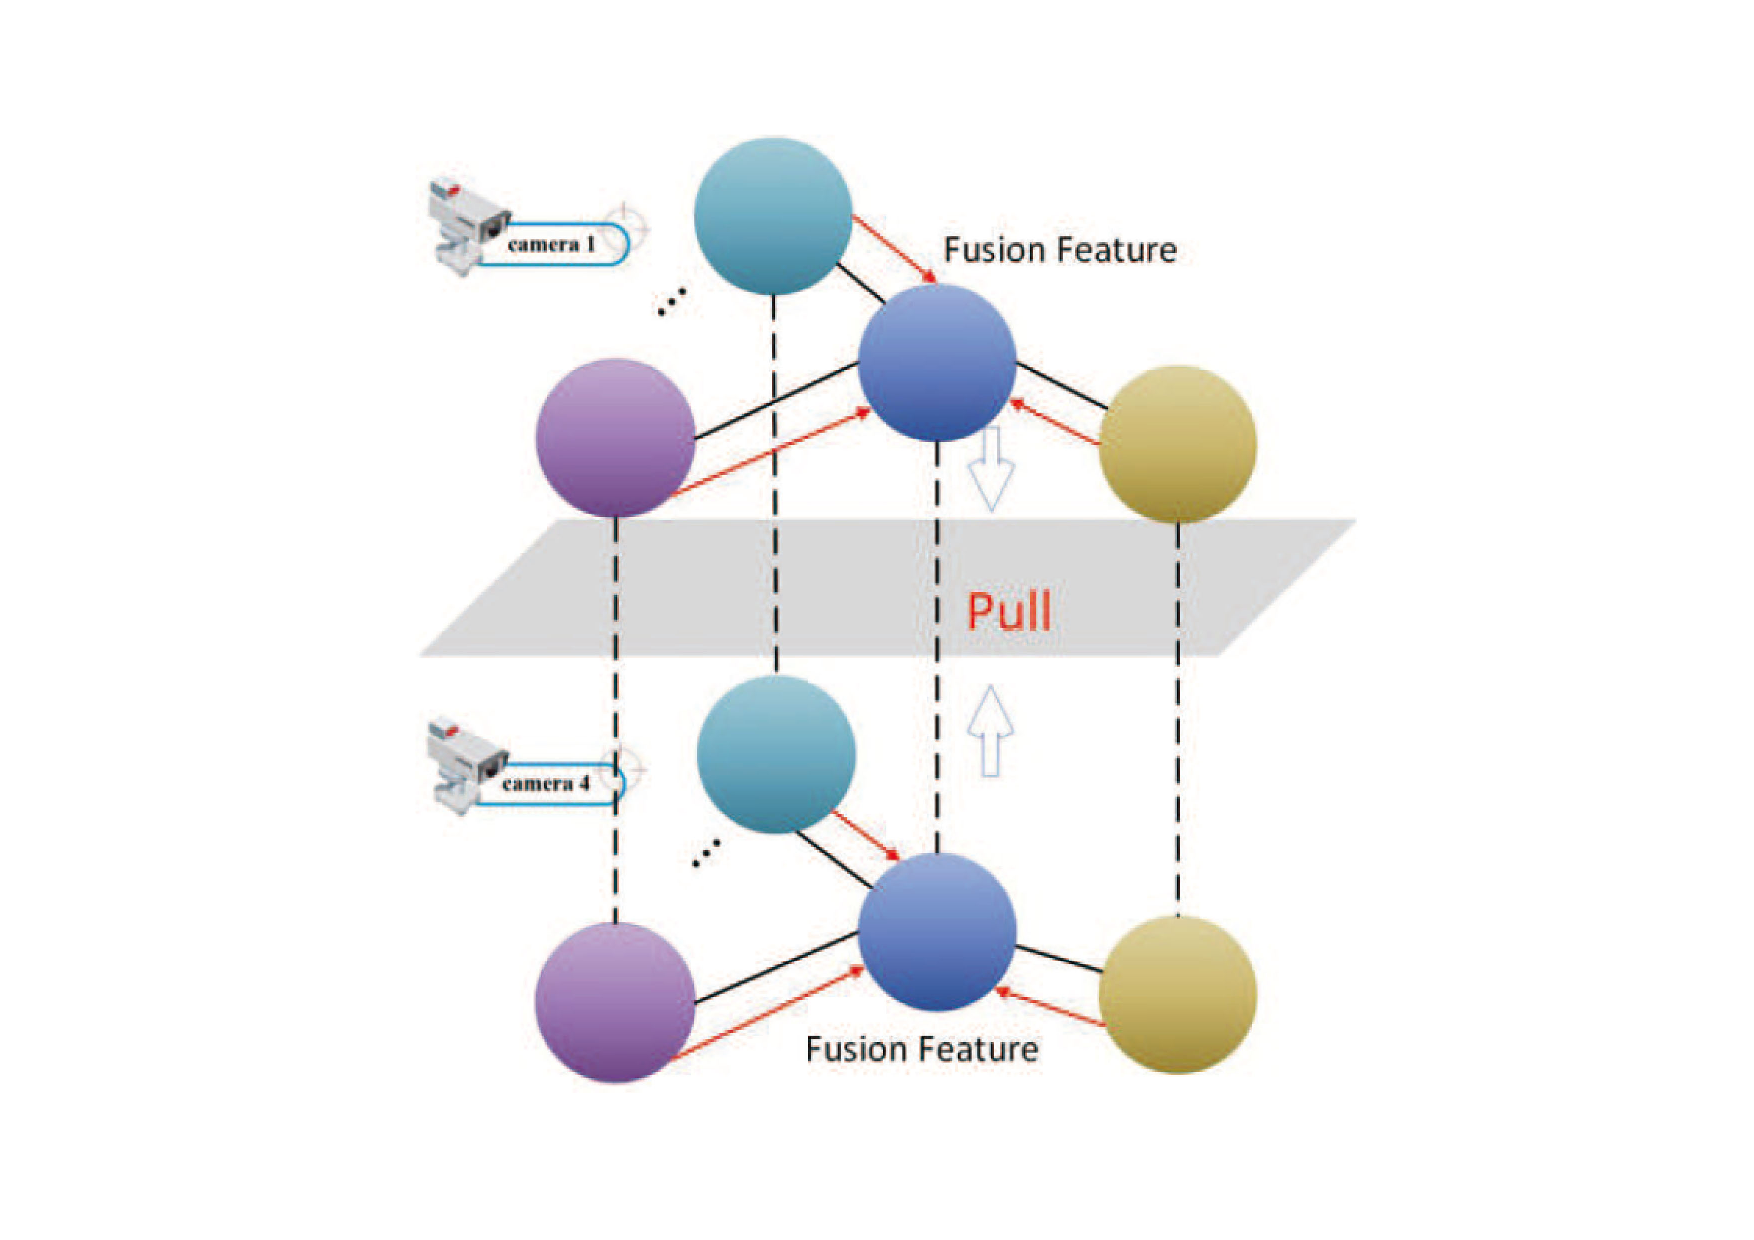
\includegraphics[scale=0.4]{fig/feature_fusion.pdf}
	\caption{An example to illustrate the principle of fusion feature generation by GCN, where two nodes with the same color under different video frames represent the same identity.
	The blue node first integrates feature representations from neighboring nodes, and then our algorithm pulls closer the nodes with same labels.}
	\label{fig:feature_fusion}
\end{figure}


\begin{figure}[ht]
	\centering
	\begin{tikzpicture}
	\draw (0,0) -- (0,4);
	\draw (2,2) circle (2);
	\end{tikzpicture}
	\caption{An example to illustrate the principle of fusion feature generation by GCN, where two nodes with the same color under different video frames represent the same identity.
	The blue node first integrates feature representations from neighboring nodes, and then our algorithm}
\end{figure}




\subsection{Training Strategy}

Different from the previous approaches, we define three kinds of samples (pseudo-positive, visually similar, and pseudo-negative) to train our model.
Given a node $v_i$, the pseudo-positive samples are defined as those that have a high condidence to be same identity with $v_i$.
Here, we set two conditions to ensure a high confidence: 
First, a pseudo-positive sample should have a similar appearance with $v_i$;
Second, the spatial neighbors between a pseudo-positive sample and $v_i$ should be well matched.
This is consistent with our manual tagging process. 
When we cannot visually identify whether two samples are the same identity, we would observe the matching degree of their neighbors for further confirmation.
Compared to pseudo-positive samples, visually similar samples only have similar appearances with respect to $v_i$, but have different neighbors.
Therefore, they have a lower confidence to be the same identity with $v_i$ as compared to pseudo-positive ones.
Pseudo-negative samples are required to have dissimilar appearances with $v_i$.
\Cref{fig:sample_difference} lists an example to illustrate the differences between pseudo-positive and visually similar samples. 

Based on these samples, we employ three loss functions to train our model.
Let $P_{v_i}$, $V_{v_i}$, and $N_{v_i}$ be sets of pseudo-positive, visually similar, and pseudo-negative samples with respect to $v_i$, respectively.
The first loss is pseudo-positive discriminative feature learning loss (PDFL), which aims to learn discriminative fusion features by pulling close $v_i$ and its pseudo-positive samples in $P_{v_i}$ (see the white arrow line in \Cref{fig:feature_fusion}).
We express it as follows:
\begin{equation} \label{equ:pdfl}
L_{PDFL}=-log \frac{\sum_{v_j \in P_{v_i}} e^{-\frac{s}{2}||f(v_i)-f(v_j)||_2 }}{\sum_{v_j \in P_{v_i}, V_{v_i}, N_{v_i} } e^{-\frac{s}{2} ||f(v_i)-f(v_j)||_2 } }, 
\end{equation}
where $s$ is the hyper-parameter.
The minimization of $L_{PDFL}$ ensures a small distance between $v_i$ and its pseudo-positive samples,
and thus the learned fusion features could well capture the characters of $v_i$.
The second loss is positive visual contrary loss (PVCL).
This function aims to distinguish pseudo-positive samples from visually similar ones, 
and we employ the triple loss to implement it as follows:
\begin{equation} \label{equ:pvcl}
\begin{aligned}
L_{PVCL}=max&\{ \frac{1}{|P_{v_i}|} \sum_{v_j \in P_{v_i} } ||f(v_i)-f(v_j)||_2 +\alpha_{pv} \\
&-\frac{1}{|V_{v_i}|} \sum_{v_j \in V_{v_i}} ||f(v_i)-f(v_j)||_2 , 0 \},
\end{aligned} 
\end{equation}
where $|\cdot|$ means quantity, $\alpha_{pv}$ is the minimum distance between the samples in $P_{v_i}$ and $V_{v_i}$, respectively.
PVCL ensures a reasonable distance between psseudo-positive and visually similar samples, 
and it helps the model identify visually similar but irrelevant samples to enhance the precision.
The third loss is positive-negative contrary loss (PNCL).
This function aims to exclude negative samples, 
and we also employ the triple loss to implement it as follows:
\begin{equation} \label{equ:pncl}
\begin{aligned}
L_{PNCL}=max&\{ \frac{1}{|P_{v_i}|} \sum_{v_j \in P_{v_i} } ||f(v_i)-f(v_j)||_2 +\alpha_{pn} \\
&-\frac{1}{|N_{v_i}|} \sum_{v_j \in V_{v_i}} ||f(v_i)-f(v_j)||_2 , 0 \},
\end{aligned} 
\end{equation}
where $\alpha_{pn}$ is the minimum distance between the samples in $P_{v_i}$ and $N_{v_i}$, respectively.
Compared to visually similar samples, pseudo-negative samples usually have a larger distance to pseudo-positive ones, 
and thus we set $\alpha_{pn} > \alpha_{pv}$ is our experiments. 
By combining the above three loss functions, the final loss function is defined as follows:
\begin{equation} \label{equ:final_loss}
L = L_{PDFL} + \lambda_1 L_{PVCL} + \lambda_2 L_{PNCL},
\end{equation}
where $\lambda_1$, $\lambda_2$ are weight parameters to control the importance of $L_{PVCL}$ and $L_{PNCL}$, respectively.

Different from the previous approaches, our approach distinguishes pseudo-positive samples from visually similar ones,
and simultaneously employs three loss functions to train the model.
Moreover, by considering both visual similarity and spatial adjacency, the generated fusion features are more discriminative, 
and thus could better identify different objects for data association in online MOT task.



\begin{figure}[ht]
	\centering
	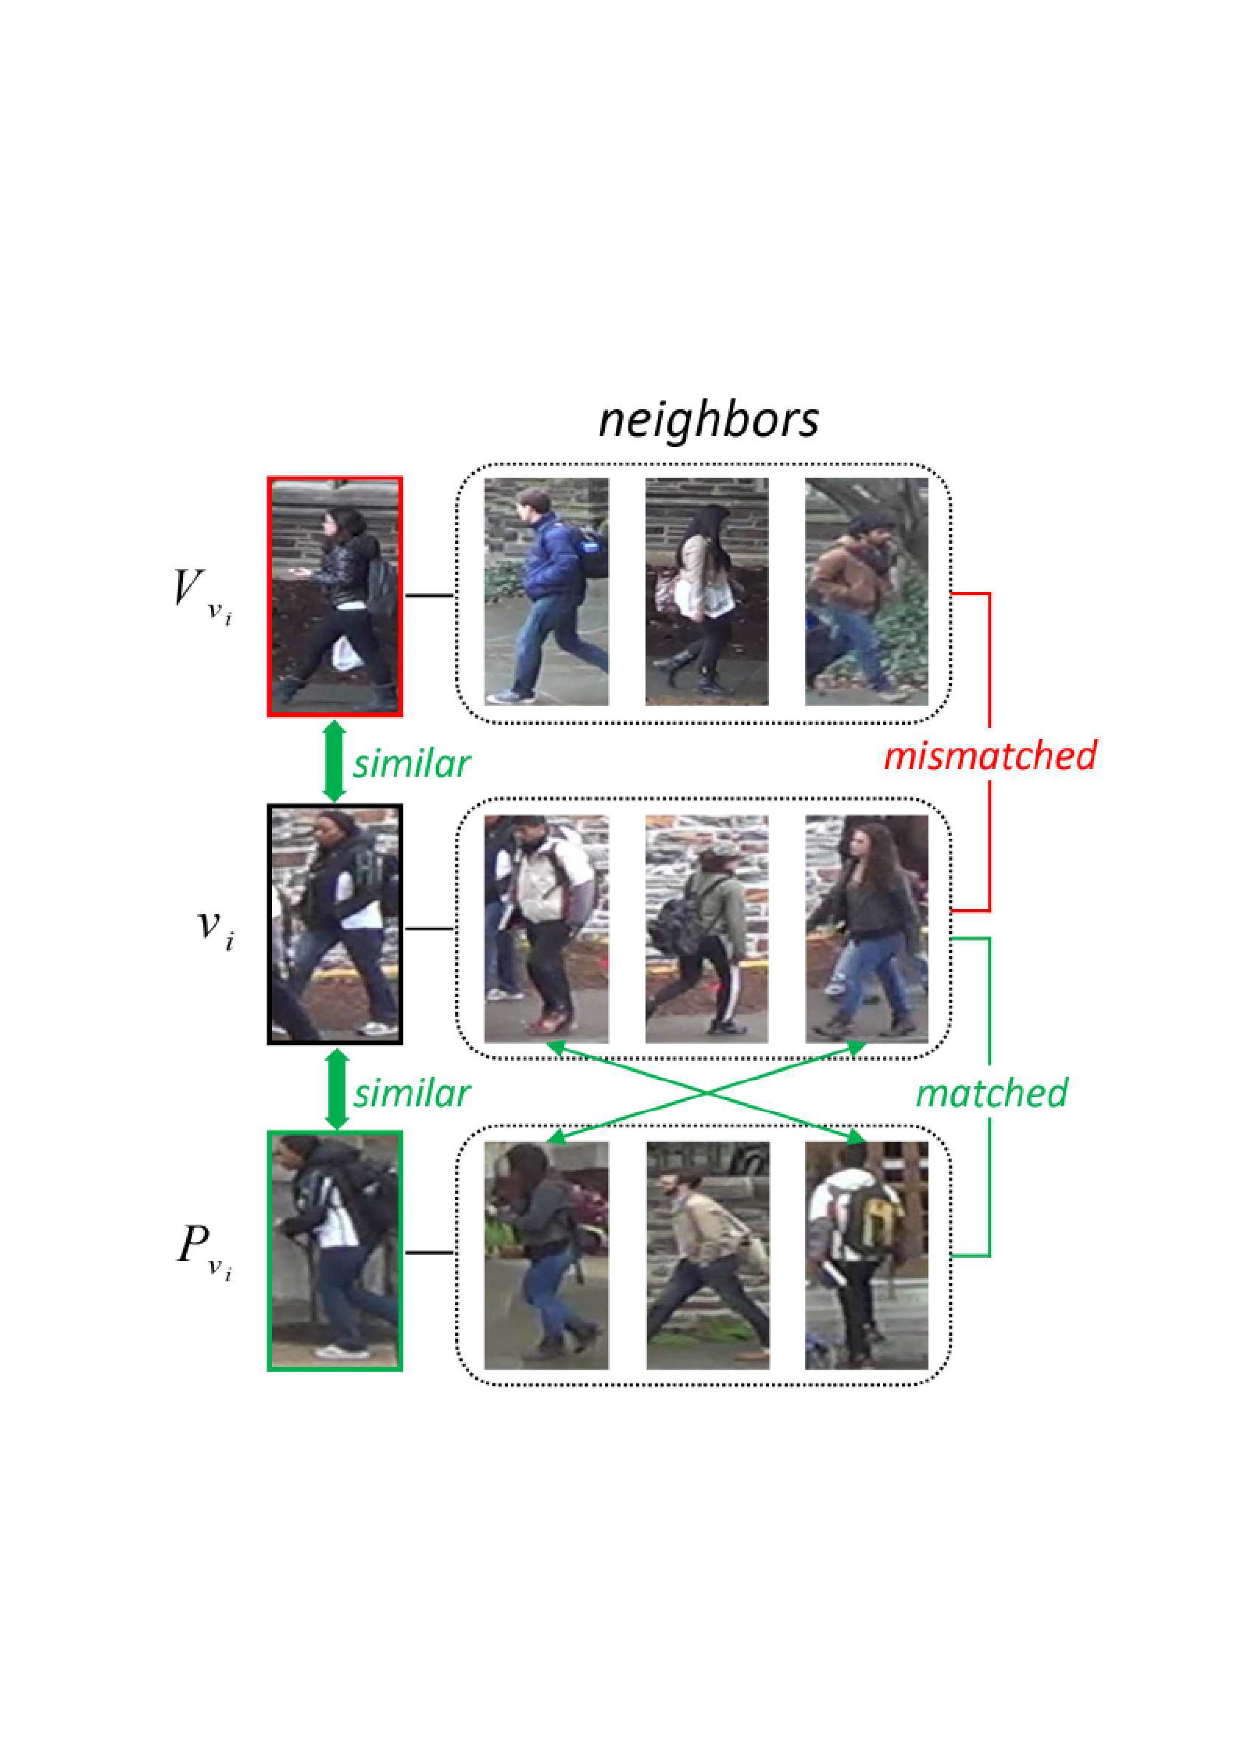
\includegraphics[scale=0.4]{fig/sample_difference.pdf}
	\caption{An example to illustrate the differences between pseudo-positive ($P_{v_i}$) and visually similar ($V_{V_i}$) samples.}
	\label{fig:sample_difference}
\end{figure}

\subsubsection{Implementation}
To implement our training process, it is required to identify $P_{v_i}$, $V_{v_i}$ and $N_{v_i}$ for each object $v_i$.
In other words, we need to explore the visual similarity and neighboring matching degree with respect to each sample, which is a time-consuming process.
To solve this problem, we devise an iterative GCN algorithm to approximately implement it.

\begin{algorithm} \label{alg:gcn}
	\caption{Iterative GCN algorithm}  
	\begin{algorithmic} % [1] show number in every line
		\Require G=(V,E): the graph;
		\State $\boldsymbol{X}$: the visual feature matrix generated by patch-based visual feature network; \\
		$\boldsymbol{F}$: the fusion feature matrix; \\
		$P_{v_i}$, $V_{v_i}$, $N_{v_i}$: the sets of pseudo-positive, visually similar, and pseudo-negative samples, respectively; \\
		$R$: the maximum number of executed epoches; \\
		$Rank(v_i,V,k,\boldsymbol{X})$: return the top $k$ similar samples from $V$ with respect to $v_i$ measured on $\boldsymbol{X}$;
		$Random(V, k)$: randomly return $k$ elements in $V$.
		\Ensure The updated fusion feature matrix $\boldsymbol{F}$. \\
		Initialize $\boldsymbol{F}=\boldsymbol{X}$
		\For{each sample $v_i$}
			\State $U_{v_i} = Rank(v_i,V,k_1+k_2, \boldsymbol{X})$
		\EndFor
		\For{$r=1$ to $R$}
			\For{each sample $v_i$}
				\State $P_{v_i}=V_{v_i}=N_{v_i}=\{\}$
				\State $P_{v_i}=Rank(v_i,U_{v_i},k_1,\boldsymbol{F})$
				\State $V_{v_i}=U_{v_i}-P_{v_i}$
				\State $N_{v_i}=Random(V-U_{v_i},k_3)$
			\EndFor
			\State Calculate the loss function in \Cref{equ:final_loss}
			\State Update $G$ by using GCN
			\State Update $\boldsymbol{F}$
		\EndFor
		
	\end{algorithmic}  
\end{algorithm}

Algorithm~\ref{alg:gcn} demonstrates the training process of our iterative GCN algorithm.
First, for each sample $v_i$, we generate a set $U_{v_i}$, which contains the most visually similar samples measured on the visual feature matrix $\boldsymbol{X}$.
Then, we calculate $P_{v_i}$, $V_{v_i}$, $N_{v_i}$ in each epoch.
Here, we make an assumption that the fusion feature matrix $\boldsymbol{F}$, which incorporates both visual and spatial relationship from neighbors, could well reflect the visual similarity and the neighboring matching degree between two samples.
Thus, we take the top $k_1$ similar elements in $U_{v_i}$ measured by $\boldsymbol{F}$ as the pseudo-positive samples, and the rest are visually similar ones. 
Finally, we calculate the loss functions based on pseudo-label samples to update the parameters of GCN for generating the new fusion feature matrix $\boldsymbol{F}$, which is used to guide the generations of the new $P_{v_i}$, $V_{v_i}$ and $N_{v_i}$ in next epoch.
This process repeats $R$ times, totally.



\subsection{Online Multiple-Ojbect Tracking}

The optimal association matrix $X^*$ produced by the optimization module contains indications for both one-to-one and object death \& birth associations. The elements in $X^*$ is not binary indicators directly but can be easily interpreted. Conforming to our training setup as detailed in Section \ref{sec:41}, each element is the result of a binary classification, where the one-to-one association is marked as positive. As a result, the one-to-one association is indicated by the largest positive value in a row, and the trajectory corresponding to this row occupies the detection denoted by the corresponding column that largest value resides in. Each one-to-one association is denoted with an indicator in $O\in {\mathbb{R}^{2}}$. Birth or death happens when a row or column contains only negative values, and each of them is marked with an indicator in $B\in {\mathbb{R}}$ and $D\in {\mathbb{R}}$. To efficiently integrate $O$, $B$, and $D$ from $X^{*}$, we follow a straightforward procedure by iteratively finding the largest element $x_{max} = x_{ij}^{*}$ in $X^{*}$. If $x_{max} > 0$, then add ${(i,j)}$ into $O$, and row $i$ as well as column $j$ is marked unavailable. Once added $x_{max}$ is negative, then all the available but un-associated rows and columns are added into $D$ and $B$. Accordingly, the final association result is given indicators in $O$, $B$, and $D$.


\section{Experiments}
In this section, we present our experimental results on 2D MOT 2015 \cite{mot15} and MOT17 \cite{mot16} benchmark datasets with ablation studies and comparisons with selected baselines. More details for the MOT benchmark are available at \textit{https://motchallenge.net}.

\begin{table*}
\caption{Tracking Performance on the MOT17 Benchmark}
\begin{center}
\resizebox{175mm}{20mm}{
\begin{tabular}{|c|c|c|c|c|c|c|c|c|c|c|}
\hline
Mode & Tracker & MOTA$\uparrow$  & MOTP$\uparrow$ & IDF1$\uparrow$ & ID Sw.$\downarrow$  & MT$\uparrow$ & ML$\downarrow$  & Frag$\downarrow$  & FP$\downarrow$  & FN$\downarrow$  \\
\hline\hline
Online & GM\underline{ }PHD \cite{GM_PHD} & 36.4 & 76.2 & 33.9 & 4,607 & 4.1$\%$ & 57.3$\%$ & 11,317 & \textbf{23,723} & 330,767 \\\hline
Online & GMPHD\underline{ }KCF \cite{GMPHD_KCF} & 39.6 & 74.5 & 36.6 & 5,811 & 8.8$\%$ & 43.3$\%$ & 7,414 & 50,903 & 284,228 \\\hline
Online & EAMTT \cite{EAMTT} & 42.6 & 76.0 & \textbf{41.8} & 4,488 & 12.7$\%$ & 42.7$\%$ & 5,720 & 30,711 & 288,474 \\\hline
Online & \textbf{Ours} & \textbf{45.5} & \textbf{76.3} & 40.5 & \textbf{4,091} & \textbf{15.6$\%$} & \textbf{40.6$\%$} & \textbf{5,579} & 25,685 & \textbf{277,663} \\\hline
\hline
\hline
Offline & MHT\underline{ }bLSTM \cite{Eccv18BilinaerLSTM} & 47.5 & 77.5 & 51.9 & 2,069 & 18.2$\%$ & 41.7$\%$ & 3,124 & 25,981 & 268,042 \\\hline
Offline & IOU17 \cite{IOU17} & 45.5 & 76.9 & 39.4 & 5,988 & 15.7$\%$ & 40.5$\%$ & 7,404 & 19,993 & 281,643 \\\hline
Offline & EDMT17 \cite{EDMT17} & 50.0 & 77.3 & 51.3 & 2,264 & 21.6$\%$ & 36.3$\%$ & 3,260 & 32,279 & 247,297 \\\hline
\end{tabular}}
\end{center}
\label{tab: MOT17}
\end{table*}

\begin{table*}
\caption{Tracking Performance on the MOT15 Benchmark}
\begin{center}
\resizebox{175mm}{10mm}{
\begin{tabular}{|c|c|c|c|c|c|c|c|c|c|c|}
\hline
Mode & Tracker & MOTA$\uparrow$  & MOTP$\uparrow$ & IDF1$\uparrow$ & ID Sw.$\downarrow$  & MT$\uparrow$ & ML$\downarrow$  & Frag$\downarrow$  & FP$\downarrow$  & FN$\downarrow$  \\
\hline\hline
Online & RMOT \cite{RMOT} & 18.6 & 69.6 & \textbf{32.6} & \textbf{684} & 5.3$\%$ & 53.3$\%$ & \textbf{1,282} & 12,473 & 36,835 \\\hline
Online & RNN\underline{ }LSTM \cite{Milan2017AAAI} & 19.0 & \textbf{71.0} & 17.1 & 1490 & 5.5$\%$ & 45.6$\%$ & 2,081 & \textbf{11,578} & 36,706 \\\hline
Online & \textbf{Ours} & \textbf{21.8} & 70.5 & 27.8 & 1488 & \textbf{9$\%$} & \textbf{40.2$\%$} & 1,851 & 11,970 & \textbf{34,587} \\\hline
\end{tabular}}
\end{center}
\label{tab: MOT15}
\end{table*}

\begin{table}
\caption{Ablation Study on the MOT17 Benchmark}
\begin{center}
\resizebox{82mm}{10mm}{
\begin{tabular}{|c|c|c|c|}
\hline
Configurations & MOTA$\uparrow$  & ID Sw.$\downarrow$  & MT$\uparrow$ \\
\hline\hline
w/o assembled supervision & 43.2 & 4275 & 14.4\% \\\hline
w/o optimization module & 38.6 & 9197 & 11.8\% \\\hline
\textbf{Full} & 45.4 & 4126 & 15.6\% \\\hline
\end{tabular}}
\end{center}
\label{tab: Ablation1}
\end{table}

\subsection{Datasets and Evaluation Metrics}
\label{sec: 51}
The evaluation metrics used on MOT benchmarks include Multiple Object Tracking Accuracy (MOTA), Multiple Object Tracking Precision (MOTP), ID F1 score (IDF1), ID Precision (IDP), ID Recall (IDR), Mostly Tracked trajectories (MT, the ratio of ground-truth trajectories that are at least 80\% covered by the tracking output), Mostly Lost trajectories (ML, the ratio of ground-truth trajectories that are at most 20\% covered by the tracking output), number of False Negatives (FN), number of False Positives (FP), number of ID Switches (ID Sw.), number of Track Fragmentations (Frag).

\subsection{Implementation Details}
All the experiments are conducted on Linux with NVIDIA GTX 2080 GPU.

\textbf{Network Details}.
Input images are first resized into $224 \times 224$.
Afterwards, the pre-trained ResNet-34~\cite{he2016deep} is used to extract the appearance feature.
The size of the FC layer in each updating module is set as 256,
and the negative slop in Leaky ReLU is set as $10^-2$.
The global variable is randomly initialized between 0 and 1, 
and its size is set as 100.
The edge feature is initialized with the Intersection over Union (IoU) between the object and the detection, 
and its size is set as 2.


\textbf{Training Details}.
To construct the graph-based fusion feature network, we set the scale parameter $\alpha=0.001$ in \Cref{equ:weight_value},
and the spatial and visual thresholds $\tau_1$, $\tau_2$ to 0.8 and 0.7, respectively.
To train the graph model, the parameters of loss function are set as follows: 
The hyper-parameter $s$ in \Cref{equ:pdfl} is $10^{-3}$, 
and $\alpha_{pv}$, $\alpha_{pn}$ in \Cref{equ:pvcl}, \Cref{equ:pncl} are 5 and 30, respectively.
The balance weights $\lambda_1$, $\lambda_2$ in \Cref{equ:final_loss} are both set to 0.3.
We adopted the stochastic gradient descent (SGD)~\cite{sutskever2013importance} to optimize the network with a monentum of 0.9.
The initial learning rate is 0.001, and then gradually reduced by multiplying a factor of 0.9 at every five epoches.
Based on the updated GCN, we reselected pseudo-positive, visually similar and pseudo-negative samples according to algorithm~\ref{alg:gcn}, where the corresponding numbers $k_1$, $k_2$, and $k_3$ are 15, 5, and 30, respectively.
After that, we recalculated the loss functions to update the parameters of GCN.
This process repeated 25 times, totally.


\subsection{Evaluation on MOT Benchmark}
\label{sec: 52}
The evaluation results on both MOT17 and MOT15 datasets are shown in Table \ref{tab: MOT17} and \ref{tab: MOT15}. The arrows in each column denote the favorable changing direction of the corresponding metric. Being the only fully end-to-end trained online tracker, we emphasize highlighting the benefits of the end-to-end training methodology as well as the GNN optimization module. To this end, we avoid excessive parameter tuning efforts during testing, and training data augmentation, as well as post-tracking performance boosting heuristics refrain in the experiments. Nevertheless, we still demonstrate competitive results with other published online trackers in both datasets. Particularly, on MOT15, we compare our results with the RNN\underline{ }LSTM \cite{Milan2017AAAI}, which is claimed the first fully end-to-end multi-object tracking method that inspires our work. As shown, we achieve favorable results on several important evaluation metrics, including 39.5\%, 12.8\%, and 3.5\% improvements on IDF1, MOTA, and MT. These improvements results from the fact we integrate the appearance affinity into the end-to-end framework and the GNN optimization module can better cope with the varying cardinality problem than RNN and LSTM.

\subsection{Ablation Study}
\label{sec: 53}
Ablation study is also conducted on the MOT17 benchmark. As shown in Table \ref{tab: Ablation1}, we demonstrate the contributions of the assembled supervision and the GNN optimization module. Specifically, the first row of the table shows the performance of the whole network trained with single supervision applied on the final association output $Y$ without assembled supervision. The second row illustrates the result of directly reasoning the association result using the affinity matrix $S$, without the following GNN optimization module. Training for this configuration is assembled on affinity matrices $A$, $M$, and $S$. The last row reports the full network. As illustrated, the full network outperforms the first-row configuration in all three metrics with 4.9\%, 3.5\%, and 7.7\% improvements, proving the merits of the assembled supervision. Comparing to the second-row configuration, the full network enlarges the improvements to 15\%, 122.9\%, and 24.4\%. Although this configuration cannot be trained with the full assembled supervision due to the absence of $Y$, the extra performance improvements still advocate the contribution of the GNN optimization module.

\section{Conclusion and Future work}
We propose an end-to-end data association model for online multi-object tracking. By jointly training the affinity learning module and the GNN optimization module, they can co-adapt collaboratively, improving the adaptivity, scalability, and accuracy of the data association model. Particular, we firstly introduce GNN in the context of solving online data association with frequent birth and death, successfully settles the irregular linear assignment formulation in a data-driven way. In this paper, we emphasize on demonstrating the efficacy of end-to-end data association and the GNN optimization module, therefore the affinity computation module is lightly designed and no performance enhancing heuristics have been employed. The performance of the method can be further enhanced in future work.

{\small
\bibliographystyle{ieeetr}
\bibliography{vsg}
}

\end{document}
